\subsubsection{Caso d’uso UC8.1.3.6: Creazione ordinamento di stringhe}
	\label{UC8.1.3.6}
	\begin{figure}[h]
		\centering
			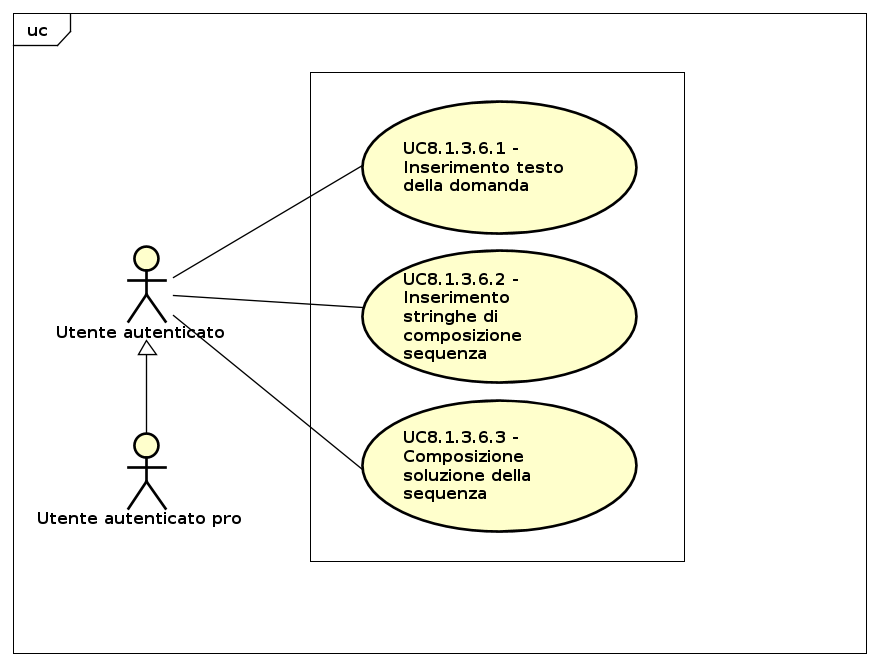
\includegraphics[scale=0.45,keepaspectratio]{UML/UC8_1_3_6.png}
		\caption{UC8.1.3.6: Creazione domanda ordinamento stringhe}
	\end{figure}
	\FloatBarrier
\begin{itemize}
	\item\textbf{Attori}: utente autenticato, utente autenticato pro;
	\item\textbf{Descrizione}: gli attori possono inserire una domanda del tipo ordinamento di stringhe;
	\item \textbf{Precondizione}: gli attori hanno selezionato la funzionalità di creazione domanda a ordinamento stringhe;
	\item\textbf{Postcondizione}: gli attori hanno creato una domanda a ordinamento di stringhe;
	\item\textbf{Scenario principale}:
		\begin{enumerate}
			\item Gli attori devono compilare il campo dati destinato alla scrittura del testo della domanda (UC8.1.3.6.1);
			\item Gli attori inseriscono le stringhe che compongono la sequenza (UC8.1.3.6.2);
			\item Gli attori indicano la sequenza esatta per identificare la soluzione (UC8.1.3.6.3);
		\end{enumerate}
\end{itemize}

\subsubsection{Caso d'uso UC8.1.3.6.1: Compilazione testo domanda}
	\begin{itemize}
		\item \textbf{Attori}: utente autenticato, utente autenticato pro;
		\item \textbf{Descrizione}: gli attori devono inserire un testo per la domanda che vogliono creare;
		\item \textbf{Precondizione}: gli attori hanno selezionato la modalità di creazione di una domanda a ordinamento di stringhe e visualizzano il wizard per l'inserimento dei dati;
		\item \textbf{Postcondizione}: gli attori hanno inserito il testo della domanda.
	\end{itemize}
	
\subsubsection{Caso d'uso UC8.1.3.6.2: Inserimento stringhe di composizione sequenza}
	\begin{itemize}
		\item \textbf{Attori}: utente autenticato, utente autenticato pro;
		\item \textbf{Descrizione}: gli attori devono inserire le stringhe che compongono la sequenza della domanda che vogliono creare;
		\item \textbf{Precondizione}: gli attori hanno inserito il testo della domanda;
		\item \textbf{Postcondizione}: gli attori hanno inserito le stringhe che compongono la sequenza.
	\end{itemize}
	
\subsubsection{Caso d'uso UC8.1.3.6.3: Composizione soluzione della sequenza}
	\begin{itemize}
		\item \textbf{Attori}: utente autenticato, utente autenticato pro;
		\item \textbf{Descrizione}: gli attori devono indicare la soluzione della sequenza della domanda che vogliono creare;
		\item \textbf{Precondizione}: gli attori hanno inserito le stringhe di sequenza;
		\item \textbf{Postcondizione}: gli attori hanno indicato la soluzione della sequenza; 
	\end{itemize}